%%%%%%%%%%%%%%%%%%%%%%%%%%%%%%%%%%%%%%%%%%%%%%%%%%%%%%%%%%%%%%%%%%%%%%%%%%%%%%%
%
% Evaluation
% 
%%%%%%%%%%%%%%%%%%%%%%%%%%%%%%%%%%%%%%%%%%%%%%%%%%%%%%%%%%%%%%%%%%%%%%%%%%%%%%%


\chapter{Results}
\label{sec:results}

\section{Results}

\newpage

\begin{figure}[H]
\centering
\subfloat[Velocity 0.01m/s]{
\includegraphics[width=0.55\textwidth]{{../images/deformationVStime/Velocity1.0}.png}
\label{fig:def1}
}
\subfloat[Velocity 0.10m/s]{
\includegraphics[width=0.55\textwidth]{{../images/deformationVStime/Velocity10.0}.png}
\label{fig:def10}
}

\subfloat[Velocity 0.20m/s]{
\includegraphics[width=0.55\textwidth]{{../images/deformationVStime/Velocity20.0}.png}
\label{fig:def20}
}
\subfloat[Velocity 0.30m/s]{
\includegraphics[width=0.55\textwidth]{{../images/deformationVStime/Velocity30.0}.png}
\label{fig:def30}
}

\subfloat[Velocity 0.50m/s]{
\includegraphics[width=0.55\textwidth]{{../images/deformationVStime/Velocity50.0}.png}
\label{fig:def50}
}
\subfloat[Velocity 3.0m/s]{
\includegraphics[width=0.55\textwidth]{{../images/deformationVStime/Velocity300.0}.png}
\label{fig:def300}
}
\caption{Time evolution of the temperature at x=y=0.4}
\label{fig:def}
\end{figure}


\section{COR}

\begin{figure}[H]
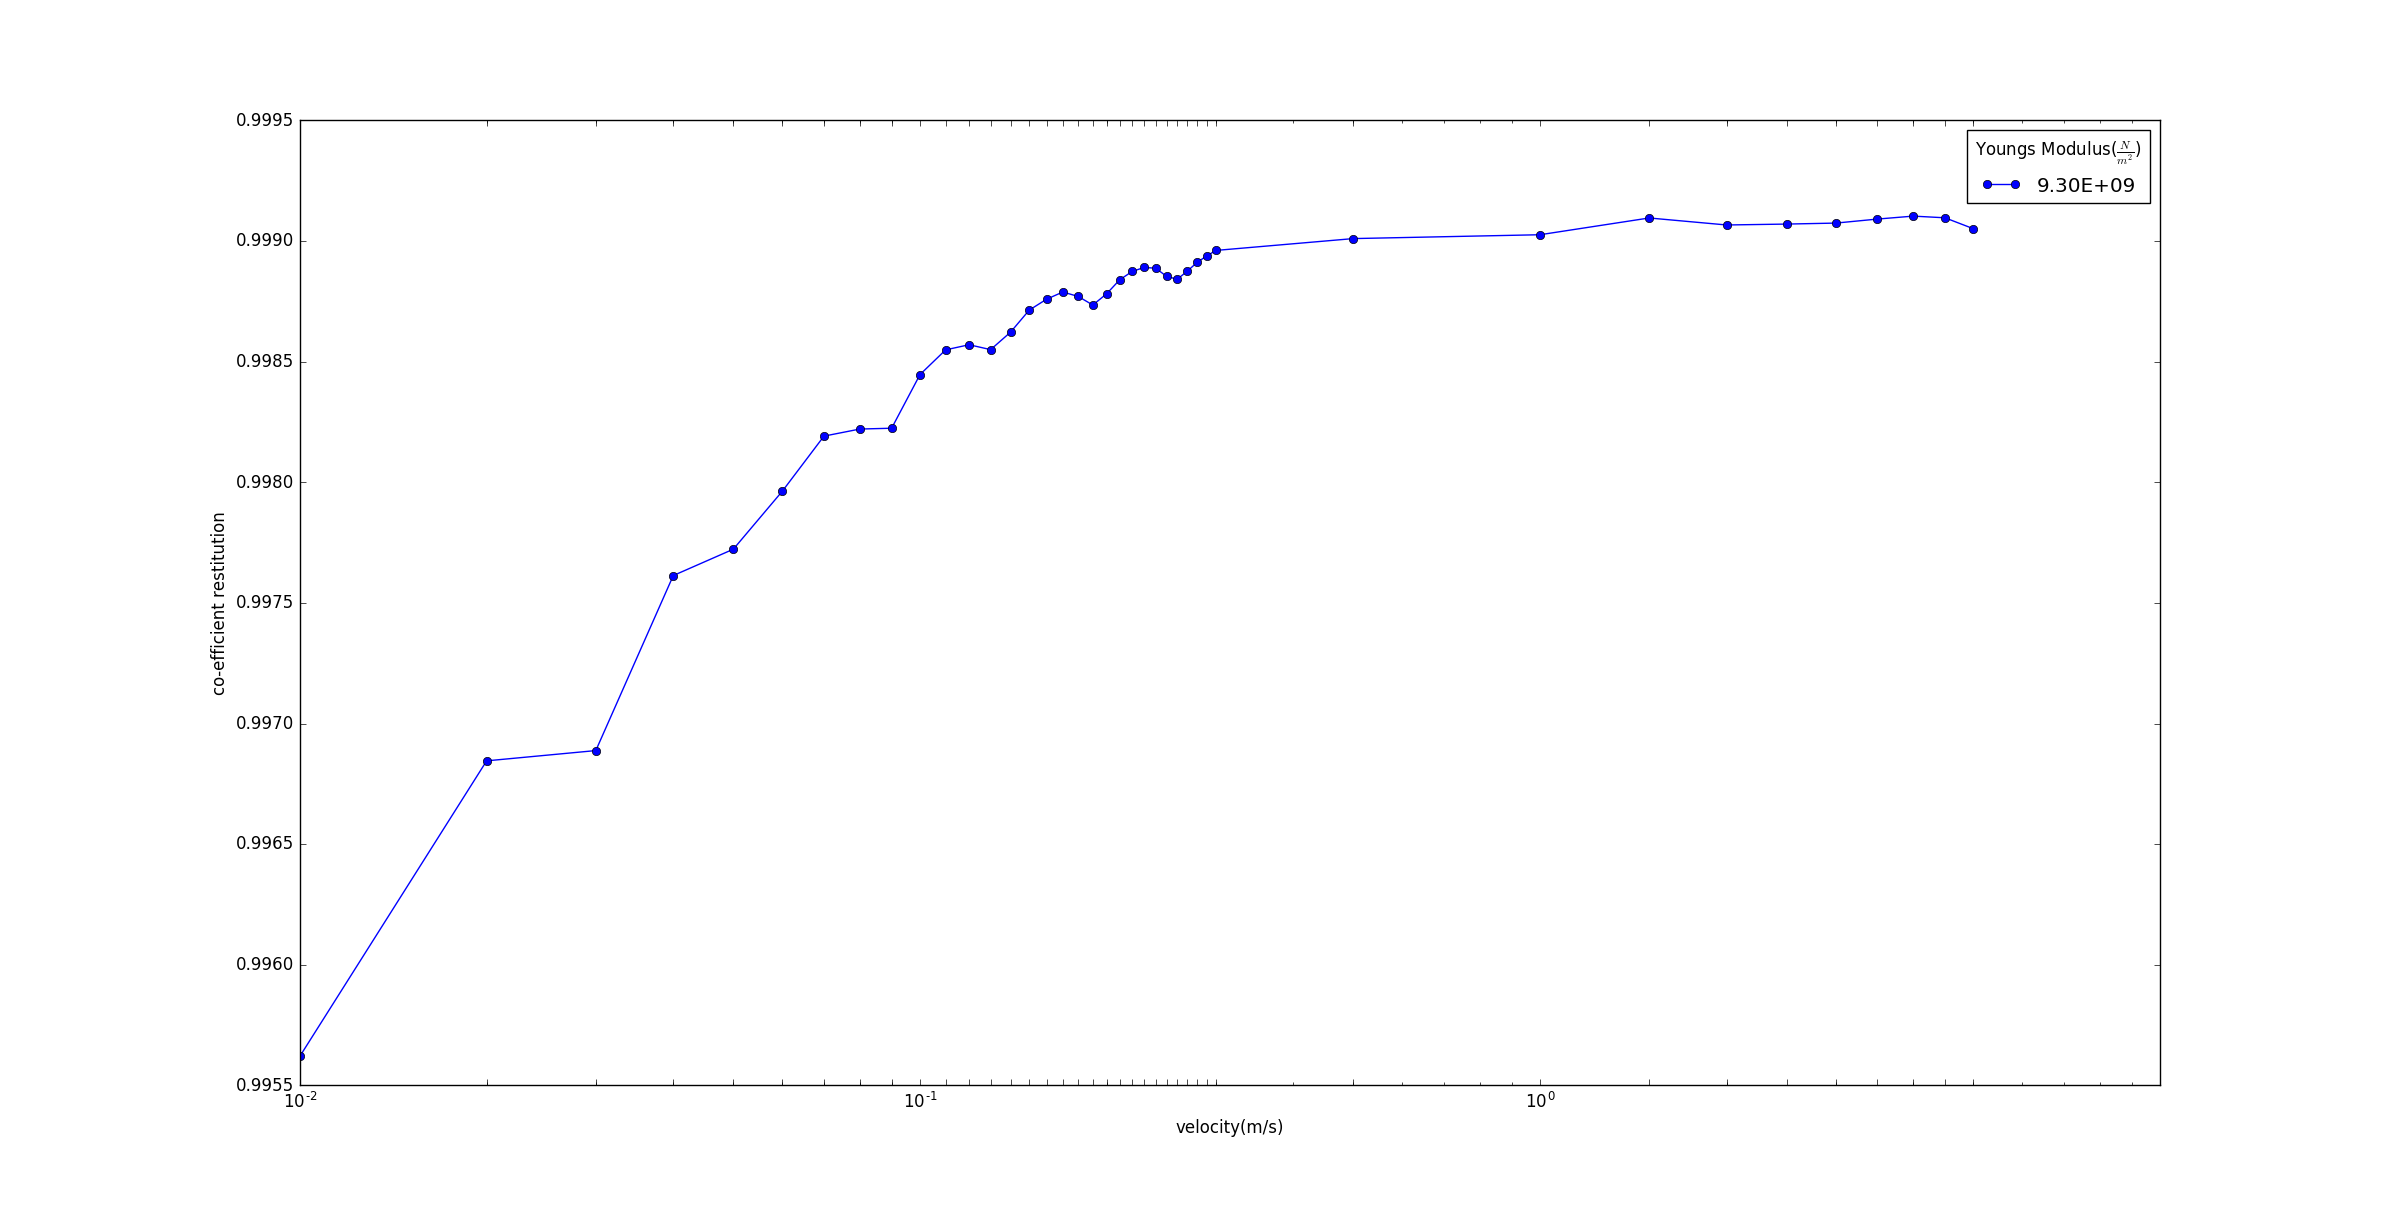
\includegraphics[width=1.0\textwidth]{../images/COR/COR.png}
\caption{COR}
\label{fig:COR}
\end{figure}


\section{Parametric Study}

\subsection{Different Youngs Modulus}

\begin{figure}[H]
\subfloat[COR]{
\includegraphics[width=1.0\textwidth]{../images/parametricStudy/COR.png}
\label{fig:CORdiffDia}
}
\end{figure}


\begin{figure}[H]
\subfloat[COR High Velocity]{
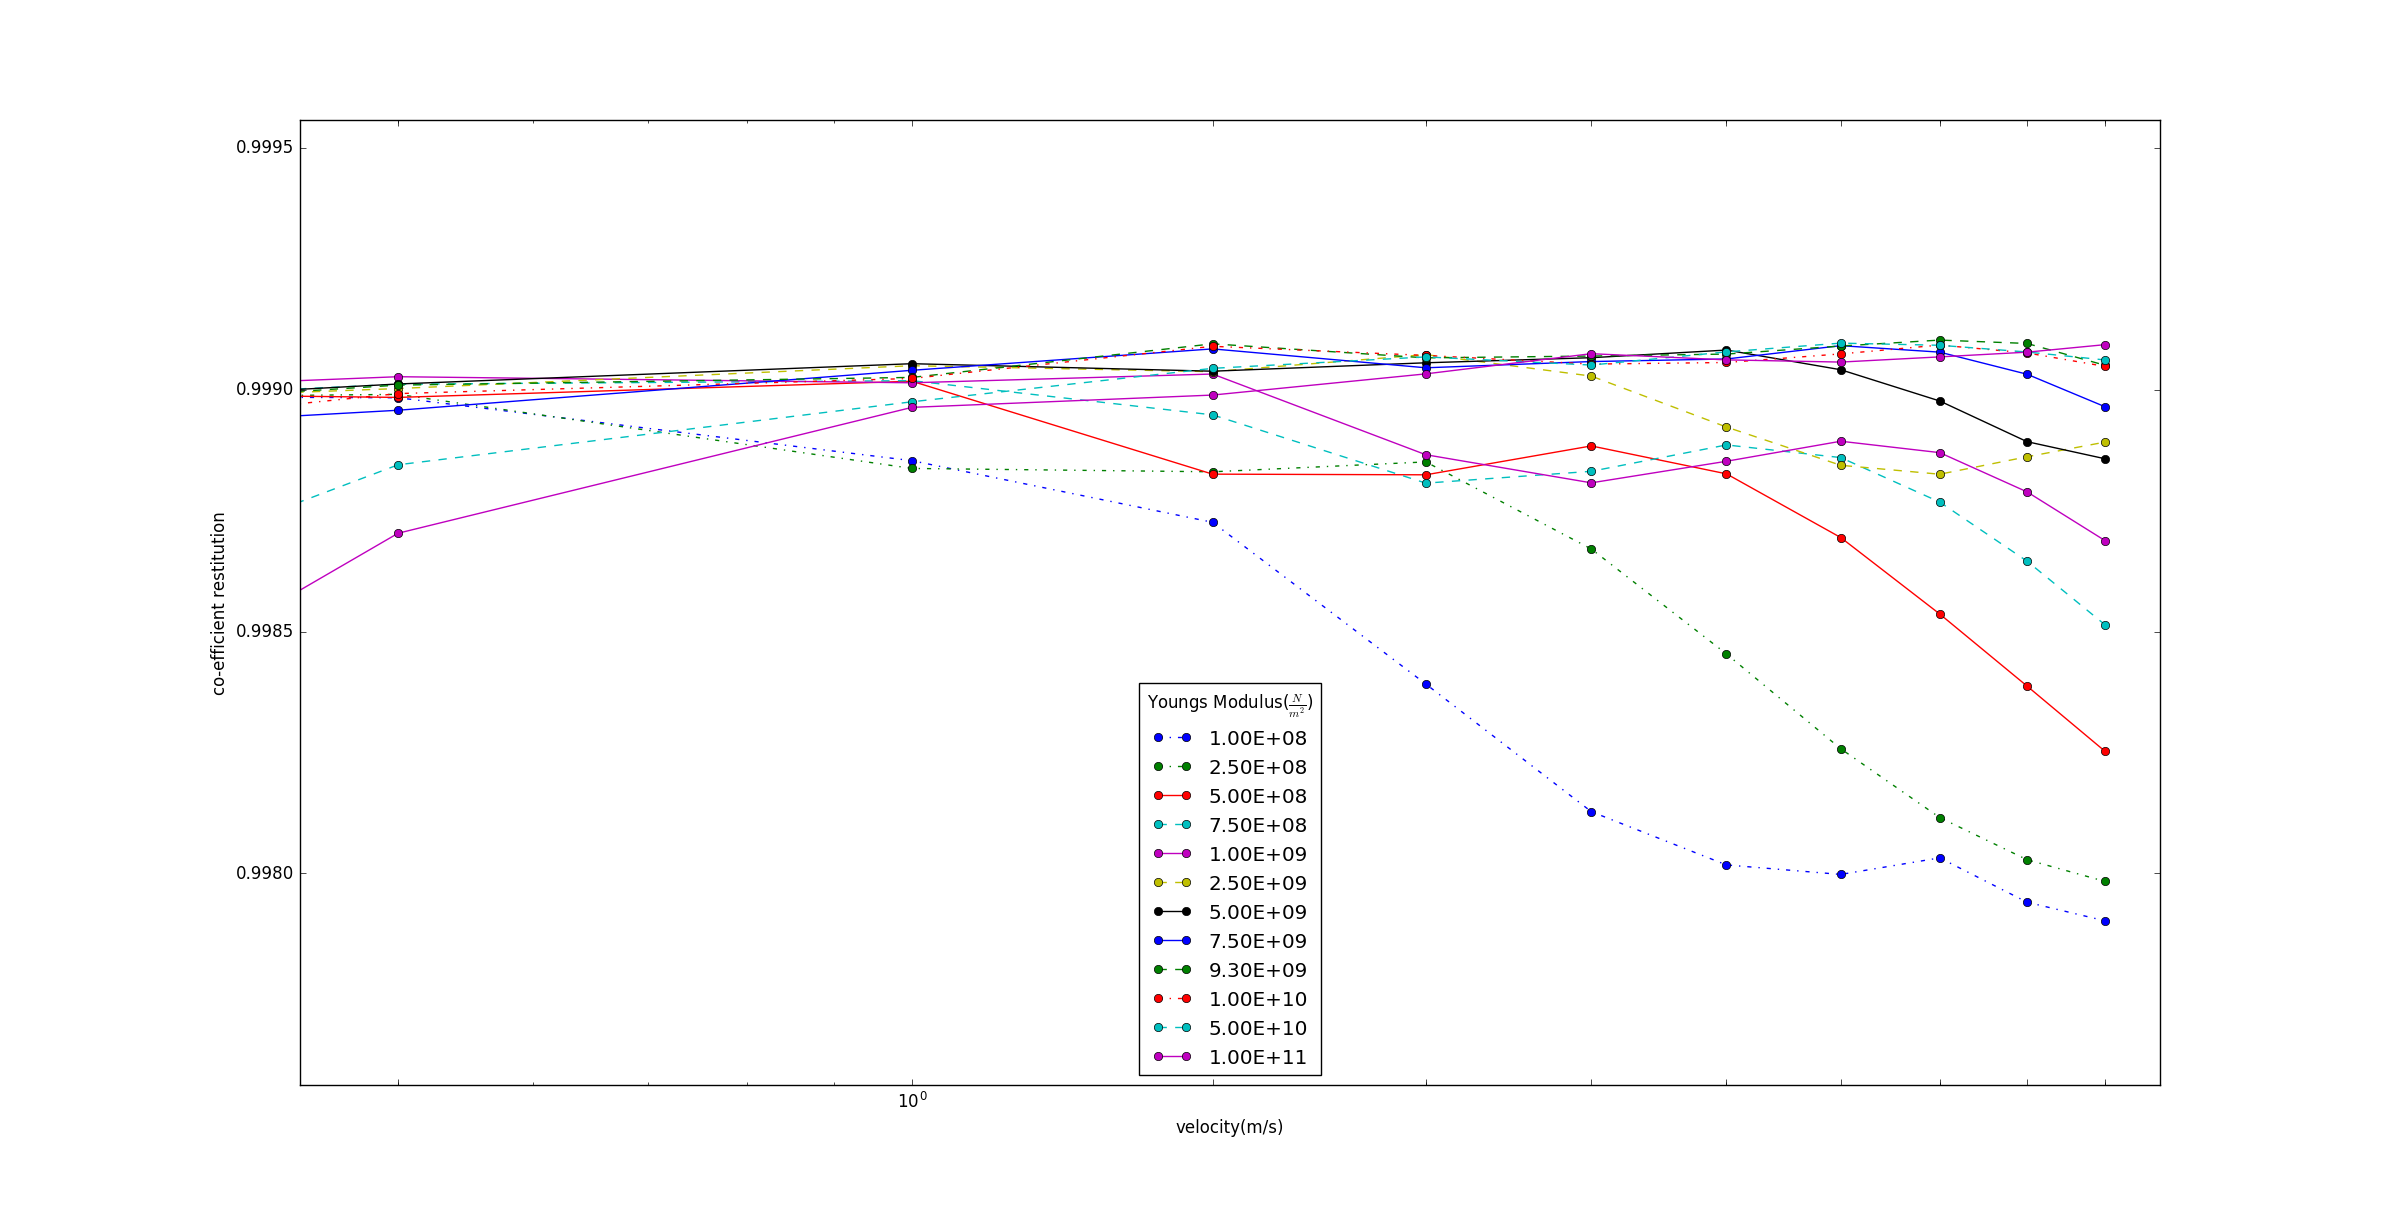
\includegraphics[width=0.55\textwidth]{../images/parametricStudy/COR_higherVEL.png}
\label{fig:CORdiffDia}
}
\subfloat[COR Low Velocity]{
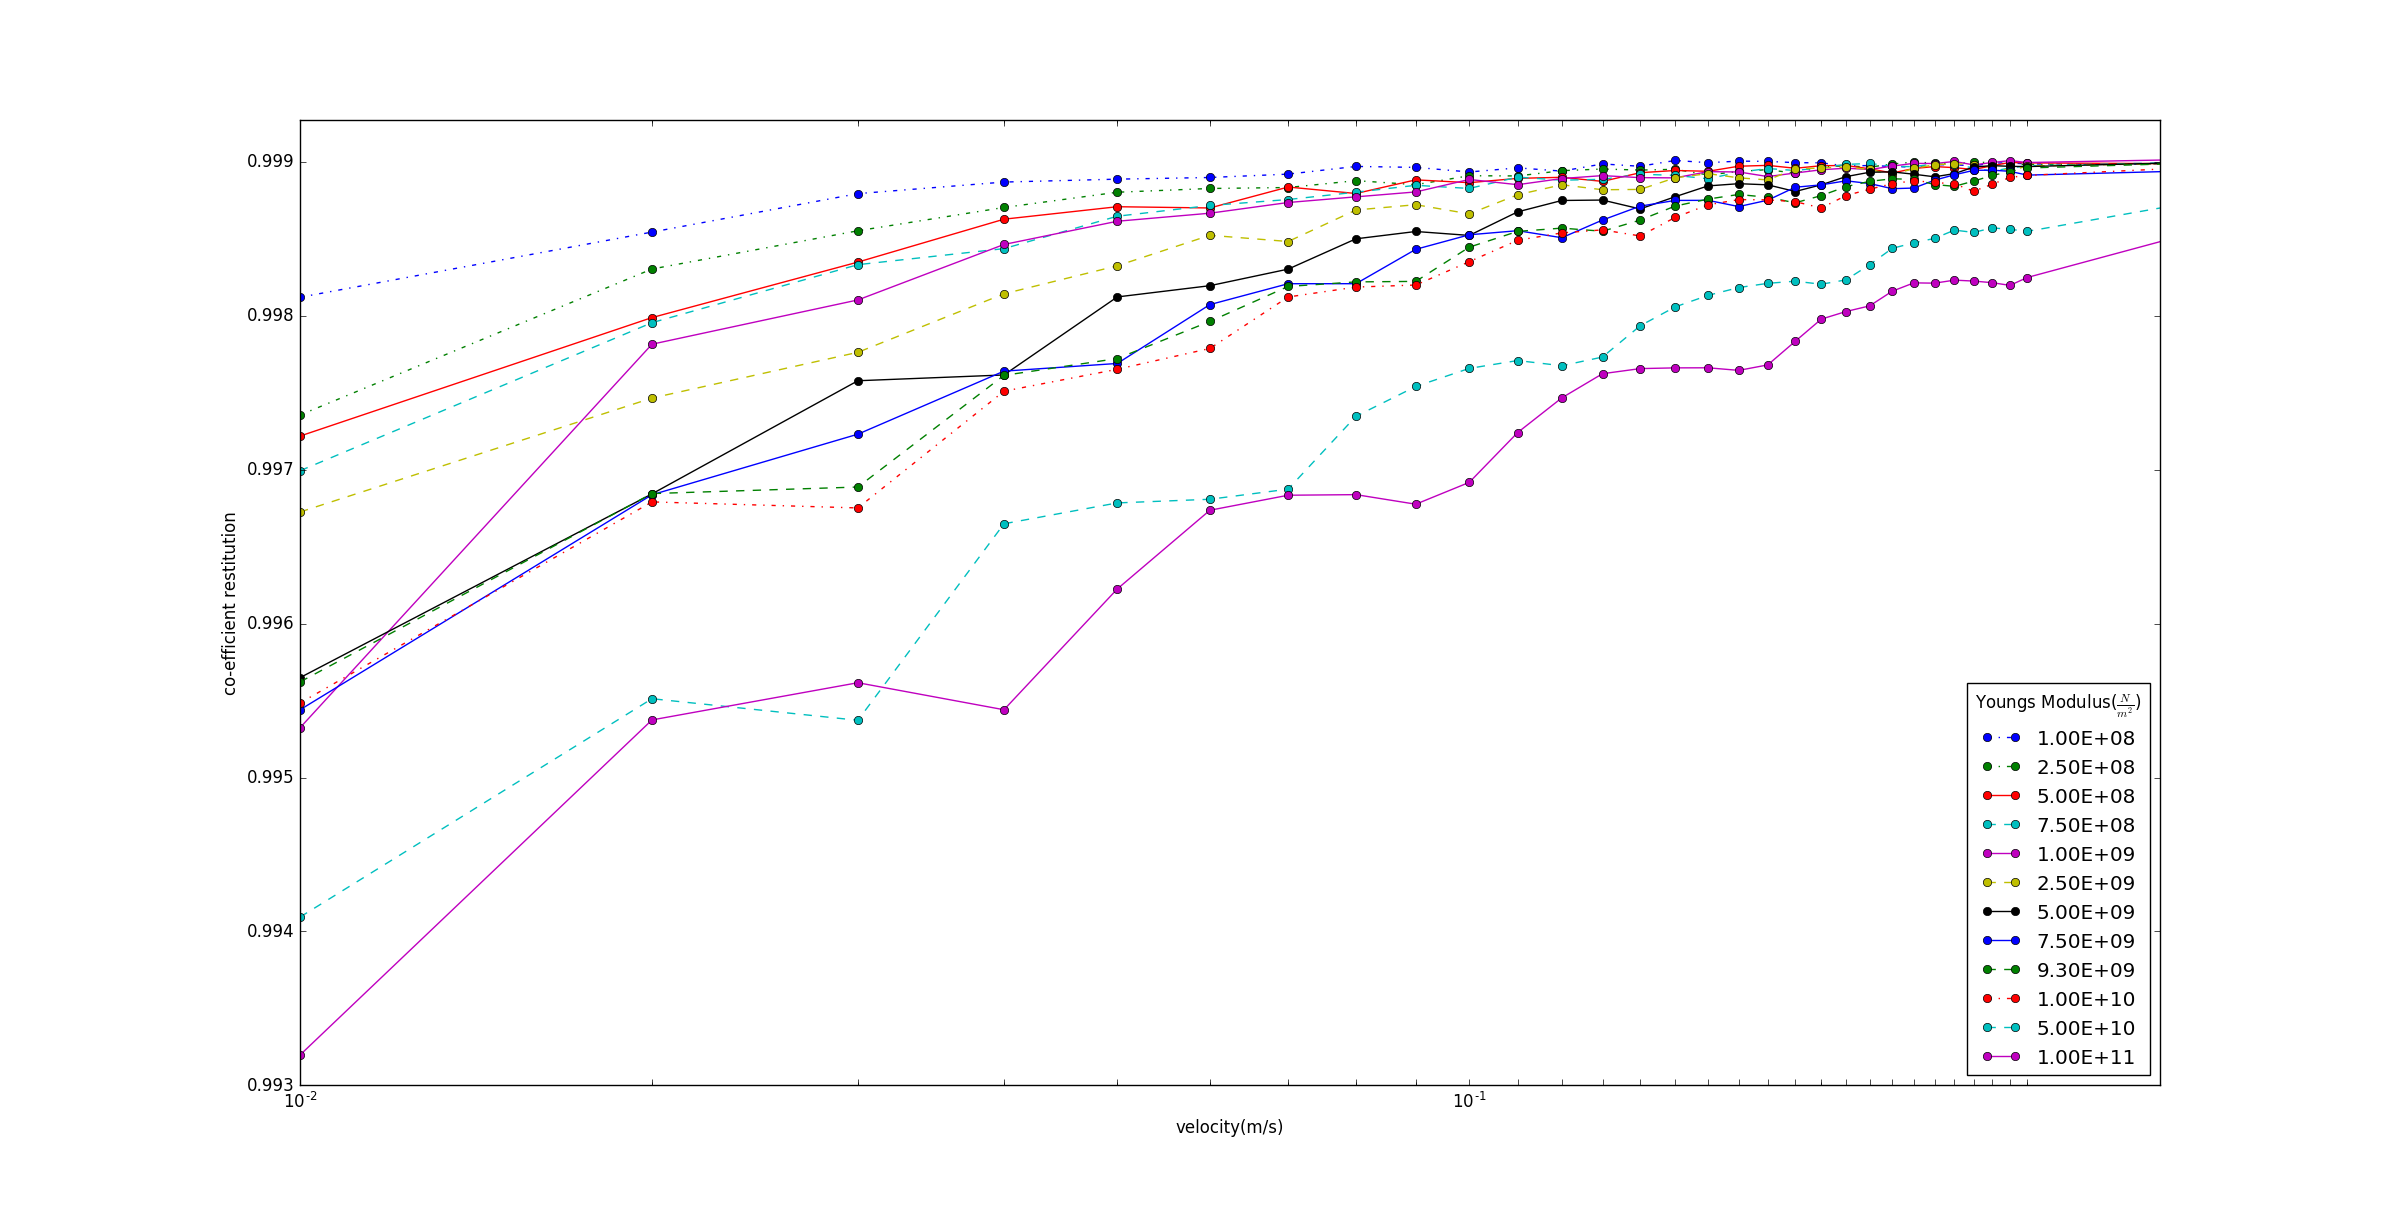
\includegraphics[width=0.55\textwidth]{../images/parametricStudy/COR_lowerVEL.png}
\label{fig:CORdiffDia}
}
\end{figure}

\subsection{Different Diameters}

\begin{figure}[H]
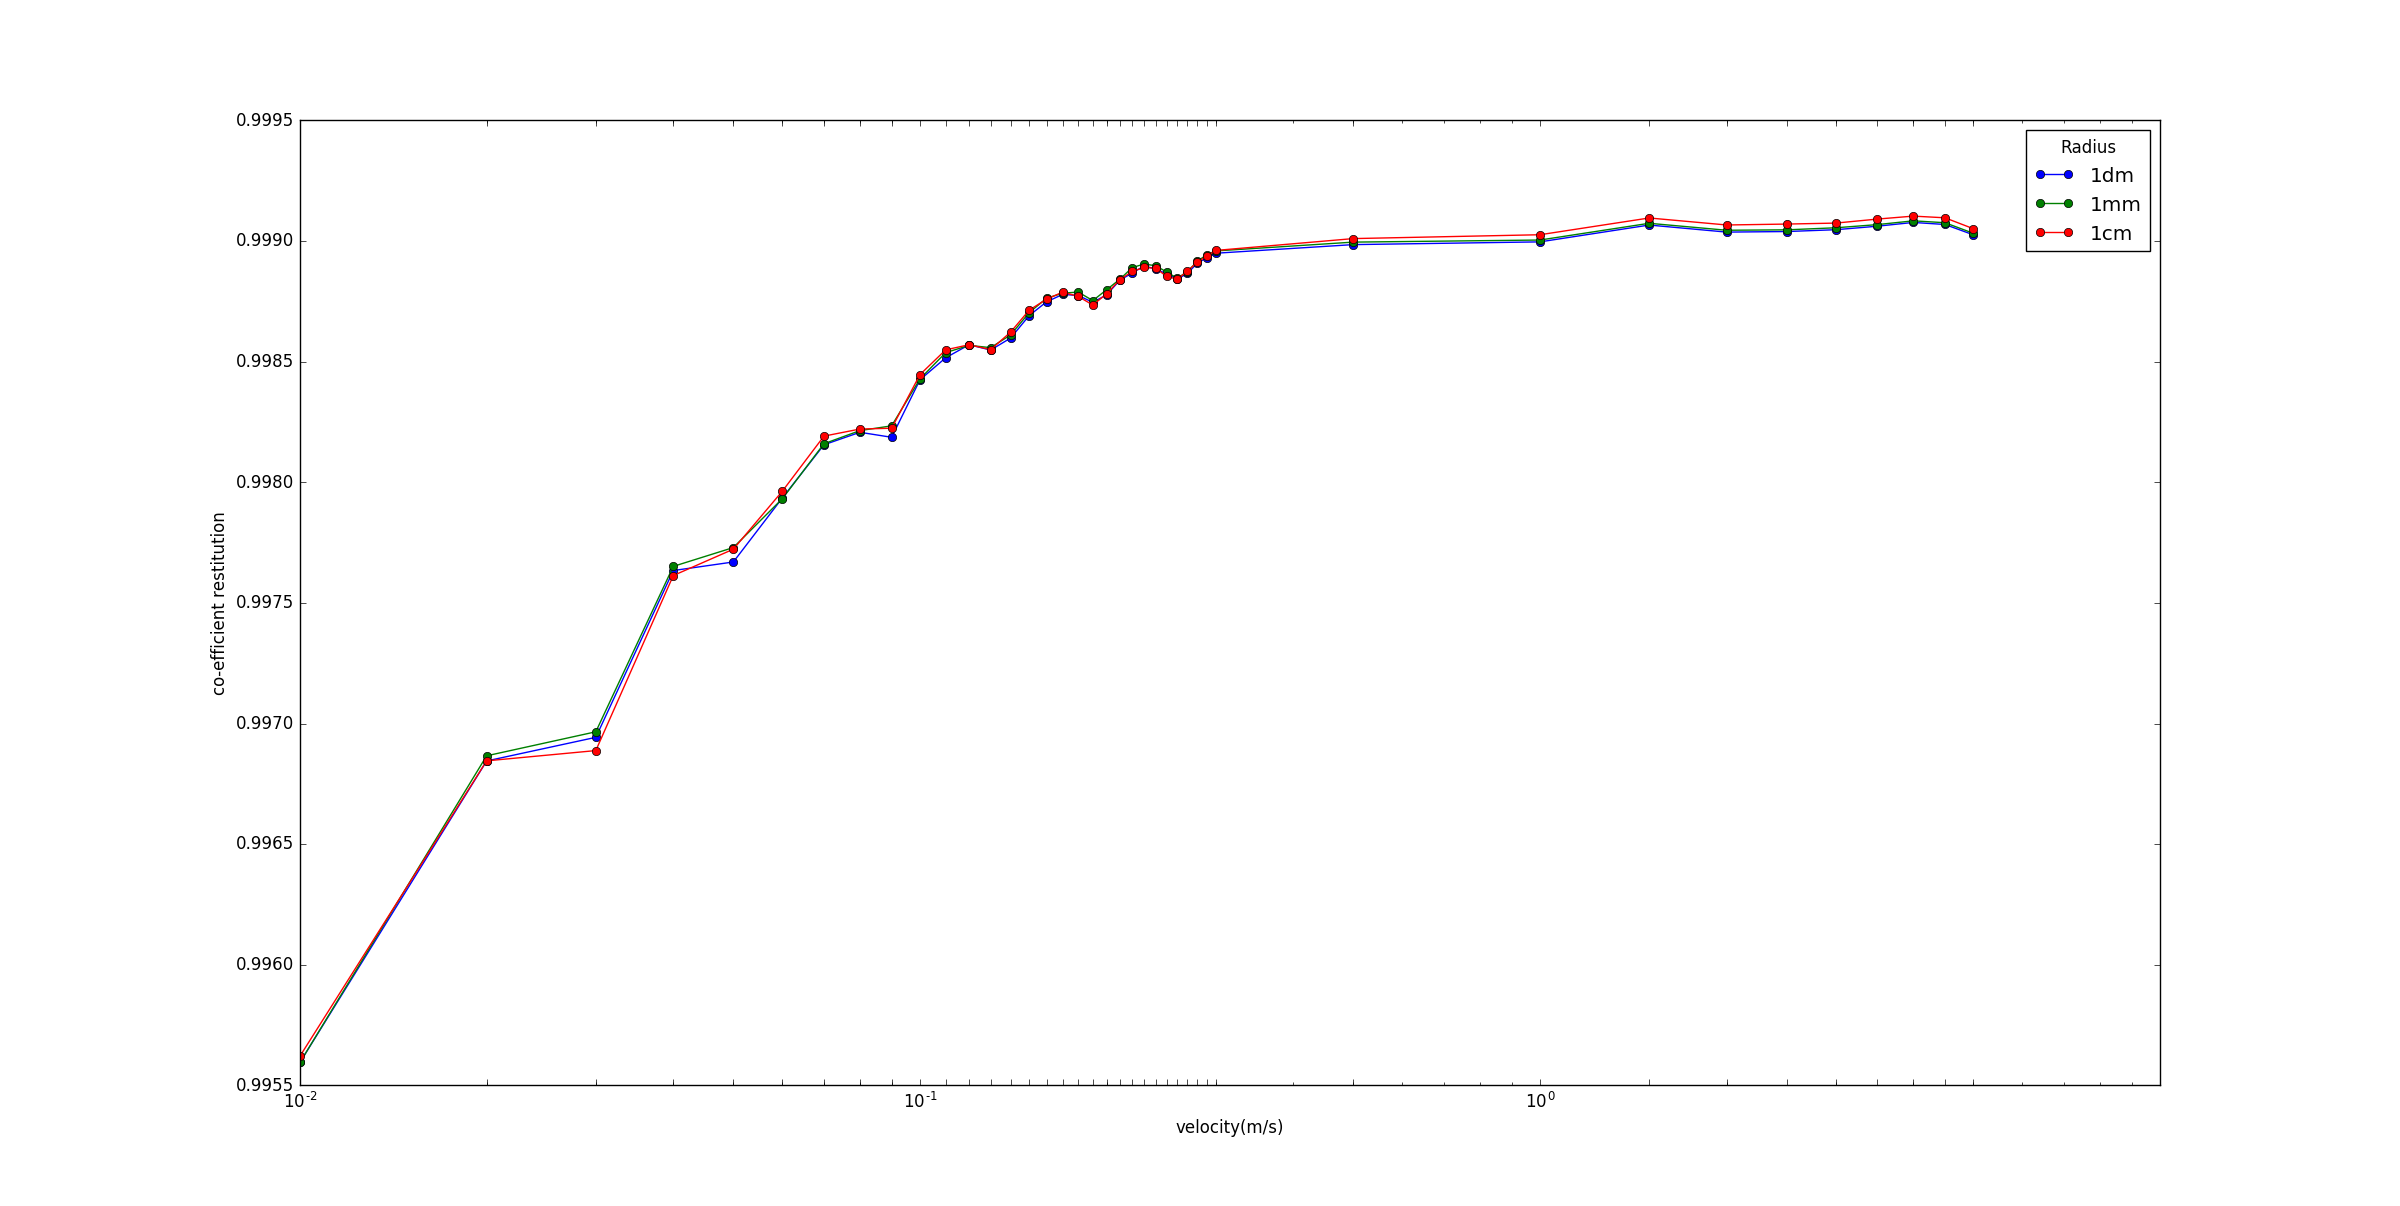
\includegraphics[width=1.0\textwidth]{../images/parametricStudy/CORvsVELdiffDAI.png}
\caption{COR}
\label{fig:COR}
\end{figure}


